\documentclass[a4paper,twoside]{article}
\usepackage{blindtext}  
\usepackage{geometry}

% Chinese support
\usepackage[UTF8, scheme = plain]{ctex}

% Page margin layout
\geometry{left=2.3cm,right=2cm,top=2.5cm,bottom=2.0cm}


\usepackage{listings}
\usepackage{xcolor}
\usepackage{geometry}
\usepackage{amsmath}
\usepackage{float}
\usepackage{hyperref}

\usepackage{graphics}
\usepackage{graphicx}
\usepackage{epsfig}
\usepackage{float}
\usepackage{caption}
\usepackage{subcaption}

\usepackage{algorithm}
\usepackage[noend]{algpseudocode}

\usepackage{booktabs}
\usepackage{threeparttable}
\usepackage{longtable}
\usepackage{tikz}
\usepackage{multicol}

% cite package, to clean up citations in the main text. Do not remove.
\usepackage{cite}

\usepackage{color,xcolor}

%% The amssymb package provides various useful mathematical symbols
\usepackage{amssymb}
%% The amsthm package provides extended theorem environments
\usepackage{amsthm}
\usepackage{amsfonts}
\usepackage{enumerate}
\usepackage{enumitem}
\usepackage{listings}
\usepackage{minted}


\usepackage{indentfirst}
\setlength{\parindent}{2em} % Make two letter space in the first paragraph
\usepackage{setspace}
\linespread{1.5} % Line spacing setting
\usepackage{siunitx}
\setlength{\parskip}{0.5em} % Paragraph spacing setting

% \usepackage[contents =22920202204622, scale = 10, color = black, angle = 50, opacity = .10]{background}

\renewcommand{\figurename}{图}
\renewcommand{\listingscaption}{代码}
\renewcommand{\tablename}{表格}
\renewcommand{\contentsname}{目录}
\floatname{algorithm}{算法}

\graphicspath{ {images/} }

%%%%%%%%%%%%%
\newcommand{\StudentNumber}{22920202204622}  % Fill your student number here
\newcommand{\StudentName}{熊恪峥}  % Replace your name here
\newcommand{\PaperTitle}{实验(四)Cache性能分析}  % Change your paper title here
\newcommand{\PaperType}{计算机系统结构实验} % Replace the type of your report here
\newcommand{\Date}{2023年5月6日}
\newcommand{\College}{信息学院}
\newcommand{\CourseName}{计算机系统结构}
%%%%%%%%%%%%%

%% Page header and footer setting
\usepackage{fancyhdr}
\usepackage{lastpage}
\pagestyle{fancy}
\fancyhf{}
% This requires the document to be twoside
\fancyhead[LO]{\texttt{\StudentName }}
\fancyhead[LE]{\texttt{\StudentNumber}}
\fancyhead[C]{\texttt{\PaperTitle }}
\fancyhead[R]{\texttt{第{\thepage}页,共\pageref*{LastPage}页}}


\title{\PaperTitle}
\author{\StudentName}
\date{\Date}

\algnewcommand\algorithmicinput{\textbf{Input:}}
\algnewcommand\algorithmicoutput{\textbf{Output:}}
\algnewcommand\Input{\item[\algorithmicinput]}%
\algnewcommand\Output{\item[\algorithmicoutput]}%

\usetikzlibrary{positioning, shapes.geometric}

\begin{document}
	
%%%%%%%%%%%%%%%%%%%%%%%%%%%%%%%%%%%%%%%%%%%%
\makeatletter % change default title style
\renewcommand*\maketitle{%
	\begin{center} 
		\bfseries  % title 
		{\LARGE \@title \par}  % LARGE typesetting
		\vskip 1em  %  margin 1em
		{\global\let\author\@empty}  % no author information
		{\global\let\date\@empty}  % no date
		\thispagestyle{empty}   %  empty page style
	\end{center}%
	\setcounter{footnote}{0}%
}
\makeatother
%%%%%%%%%%%%%%%%%%%%%%%%%%%%%%%%%%%%%%%%%%%%
	
	
\thispagestyle{empty}

\vspace*{1cm}

\begin{figure}[htb]
	\centering
	
\includegraphics[width=4.0cm]{logo.png}
\end{figure}

\vspace*{1cm}

\begin{center}
	\Huge{\textbf{\PaperType}}
	
	\Large{\PaperTitle}
\end{center}

\vspace*{1cm}

\begin{table}[H]
	\centering	
	\begin{Large}
		\renewcommand{\arraystretch}{1.5}
		\begin{tabular}{p{3cm} p{5cm}<{\centering}}
			姓\qquad 名 & \StudentName  \\
			\hline
			学\qquad号 & \StudentNumber \\
			\hline
			日\qquad期 & \Date  \\
			\hline
			学\qquad院 & \College  \\
			\hline
			课程名称 & \CourseName  \\
			\hline
		\end{tabular}
	\end{Large}
\end{table}

\newpage

\title{
	\Large{\textcolor{black}{\PaperTitle}}
}
	
	
\maketitle
	
\tableofcontents
 
\newpage
\setcounter{page}{1}

\begin{spacing}{1.2}

\section{补充实验}

\subsection{实验目的}

简单设计实验,理解Cache预取

\subsection{实验结果}

Cache预取的思路是发生未命中时将本块和下一块都调入Cache。
为了进行实验,首先需要对Cache块大小进行配置。首先,进行如下配置:
\begin{enumerate}
	\item Cache大小:4KB
	\item 相联方式:直接相联
	\item 块大小:16B
\end{enumerate}
确定Cache参数,主要是为了确定块大小。确定了块大小,就可以构造访问序列。
例如如图~\ref{fig:addrin}序列,它的访问方式如图~\ref{fig:addracc}可以看到,访问序列中,每次访问都是下一块的第一个字节。
因此,如果没有预取,Cache不会命中。通过预取,可以将下一块也调入Cache,这样就可以减少未命中次数。
% \inputminted[firstline=14,lastline=27]{python}{../code/addr.din}
\begin{figure}[htb]
	\centering
	\begin{subfigure}{0.4\textwidth}
		\centering
		\caption{访问方式}
		\label{fig:addrin}
		\inputminted{python}{../code/addr.din}
	\end{subfigure}
	\begin{subfigure}{0.4\textwidth}
		\centering
		\caption{访问位置}
		\label{fig:addracc}
		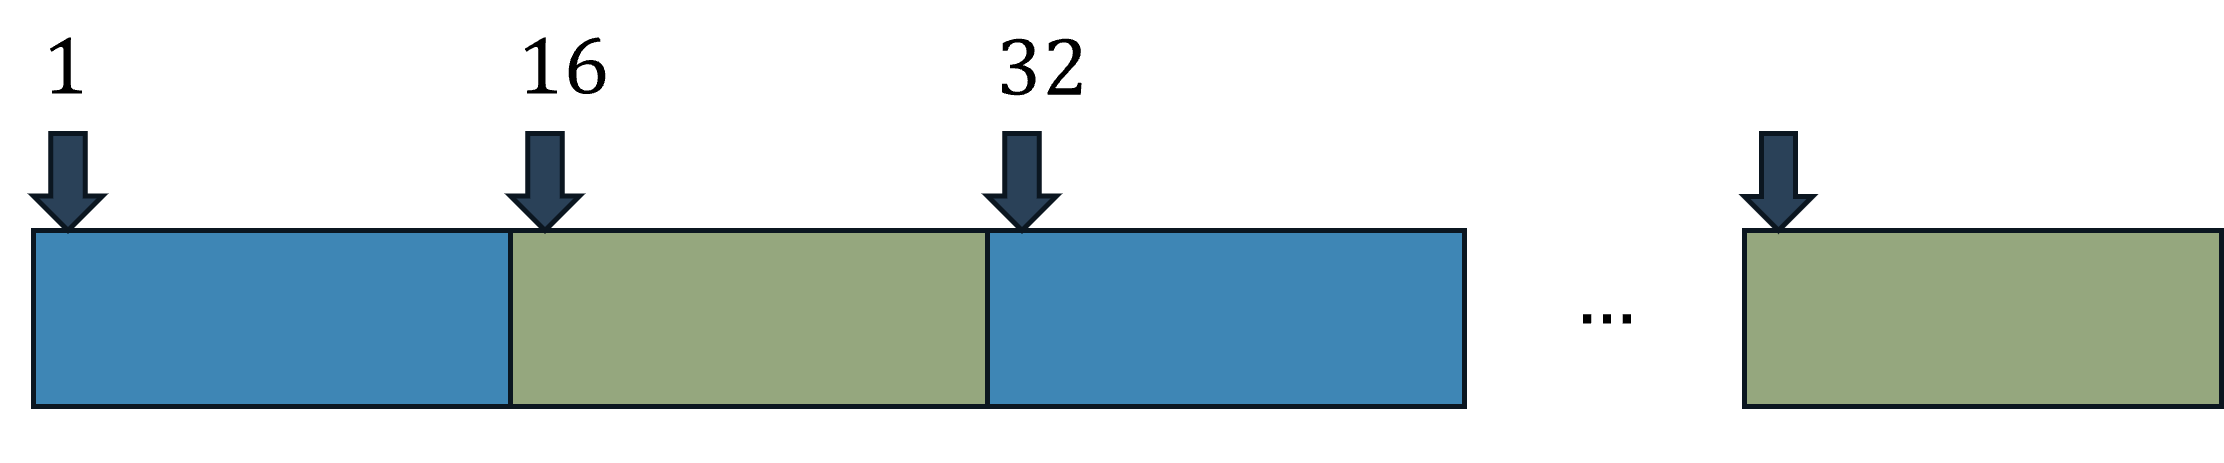
\includegraphics[width=0.9\textwidth]{pattern.png}
	\end{subfigure}
	\caption{访问地址序列}
\end{figure}

实验结果如图~\ref{fig:address},可见未命中率确实减少了。
\begin{figure}[htb]
	\centering
	\begin{subfigure}{0.4\textwidth}
		\centering
		\caption{不预取}
		\label{fig:p}
		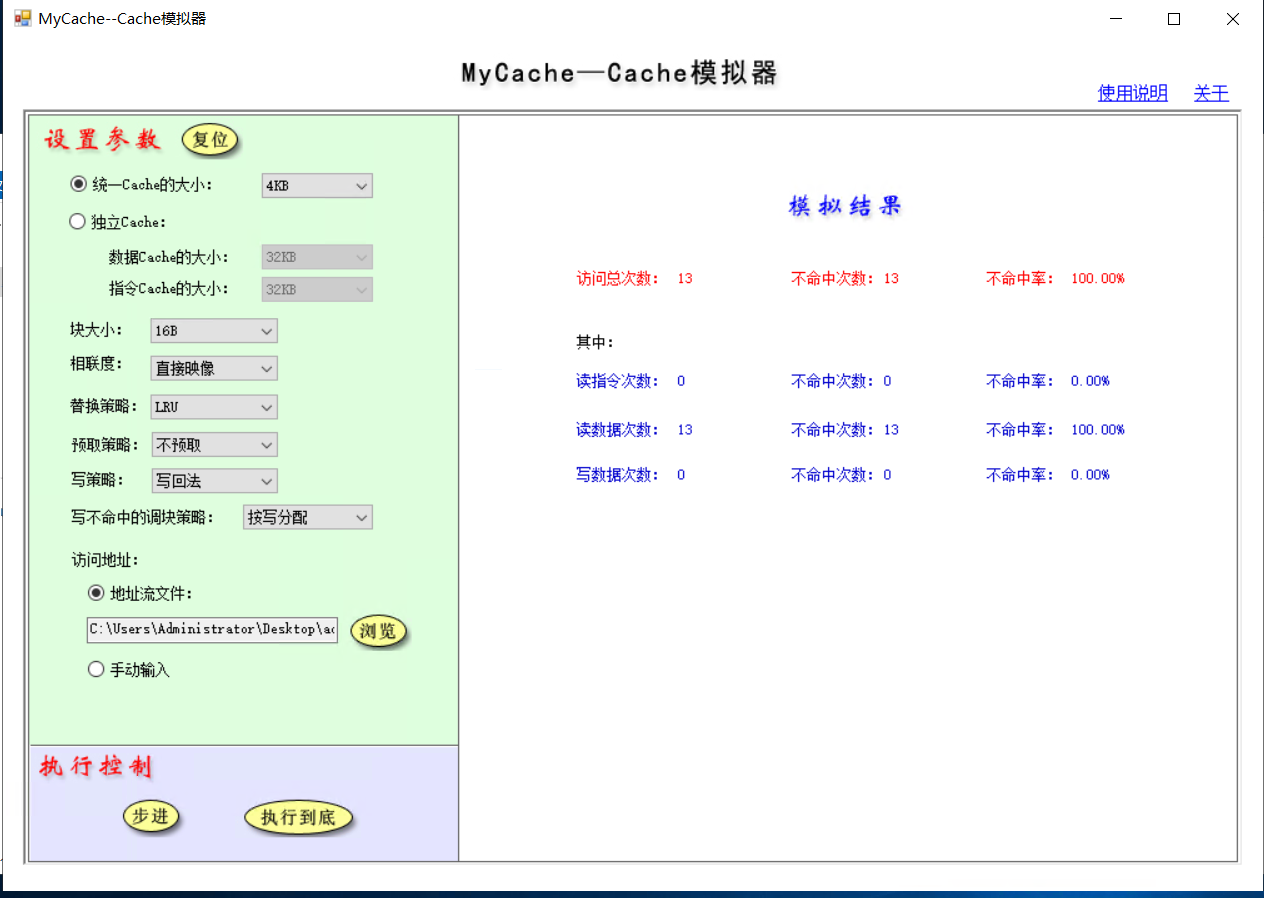
\includegraphics[width=0.9\textwidth]{p.png}
	\end{subfigure}
	\begin{subfigure}{0.4\textwidth}
		\centering
		\caption{预取}
		\label{fig:np}
		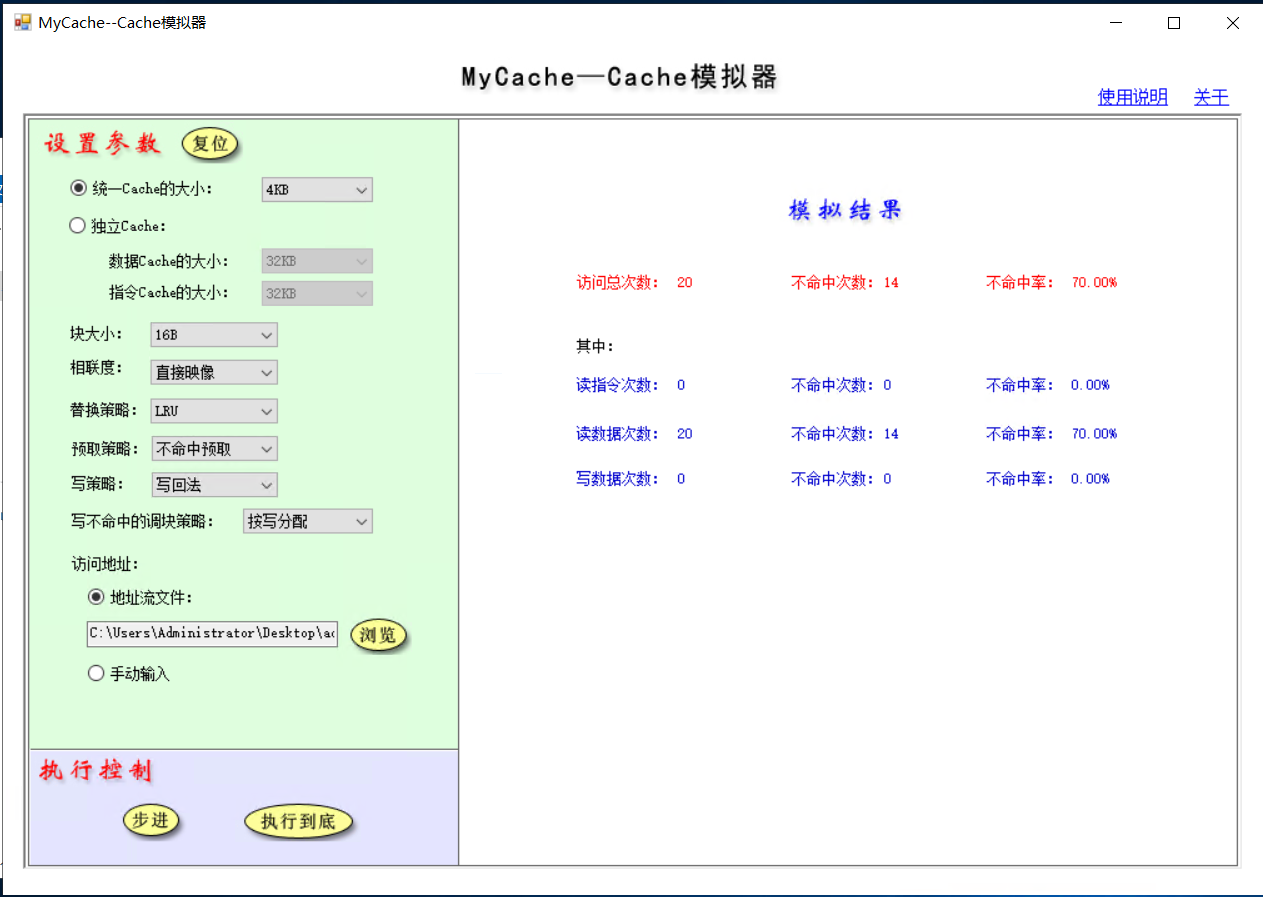
\includegraphics[width=0.9\textwidth]{np.png}
	\end{subfigure}
	\caption{实验结果}
	\label{fig:address}
\end{figure}

\subsection{分析}

虽然在本例中确实降低了未命中率,但是这种预取方式并不总是能提高性能。
例如如果下次访问不落在下一块内,这样的地址序列会导致预取过程读入无用的数据,
反而增加了额外的开销。因此,预取对性能是否有提升需要根据实际情况进行分析。

\section{探究性实验}

\subsection{实验目的}

从Cache的角度,分析以下代码的效率,以及改进方法:
\begin{minted}{c}
for(i=0;i<n;i++)
  for(j=0;j<n;j++)
    for(k=0;k<n;k++)
      C[i][j]+=A[i][k]*B[k][j];
\end{minted}

\subsection{实验结果}

可以通过重排循环的方式,使得Cache的命中率提高。如图~\ref{fig:codes}。
\begin{figure}[htb]
	\centering
	\begin{subfigure}{0.4\textwidth}
		\centering
		\caption{\texttt{ijk}}
		\inputminted{c}{../code/ijk.c}
	\end{subfigure}
	\begin{subfigure}{0.4\textwidth}
		\centering
		\caption{\texttt{ikj}}
		\inputminted{c}{../code/ikj.c}
	\end{subfigure}
	\caption{不同的循环次序}
\end{figure}

其中图~\ref{fig:ijk}是题目中所给的\texttt{ijk}次序,而图~\ref{fig:ikj}是重排过后效果较好的
\texttt{ikj}次序。实验结果如图~\ref{fig:res},可见重排后的效果确实更好。
\begin{figure}[H]
	\centering
	\begin{subfigure}{0.4\textwidth}
		\centering
		\caption{\texttt{ijk}}
		\label{fig:ijk}
		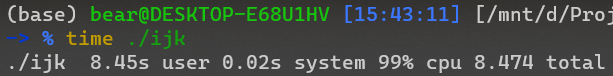
\includegraphics[width=0.9\textwidth]{ijk.png}
	\end{subfigure}
	\begin{subfigure}{0.4\textwidth}
		\centering
		\caption{\texttt{ikj}}
		\label{fig:ikj}
		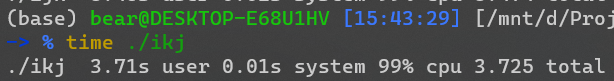
\includegraphics[width=0.9\textwidth]{ikj.png}
	\end{subfigure}
	\begin{subfigure}{0.8\textwidth}
		\centering
		\caption{对比}
		\label{fig:cmp}
		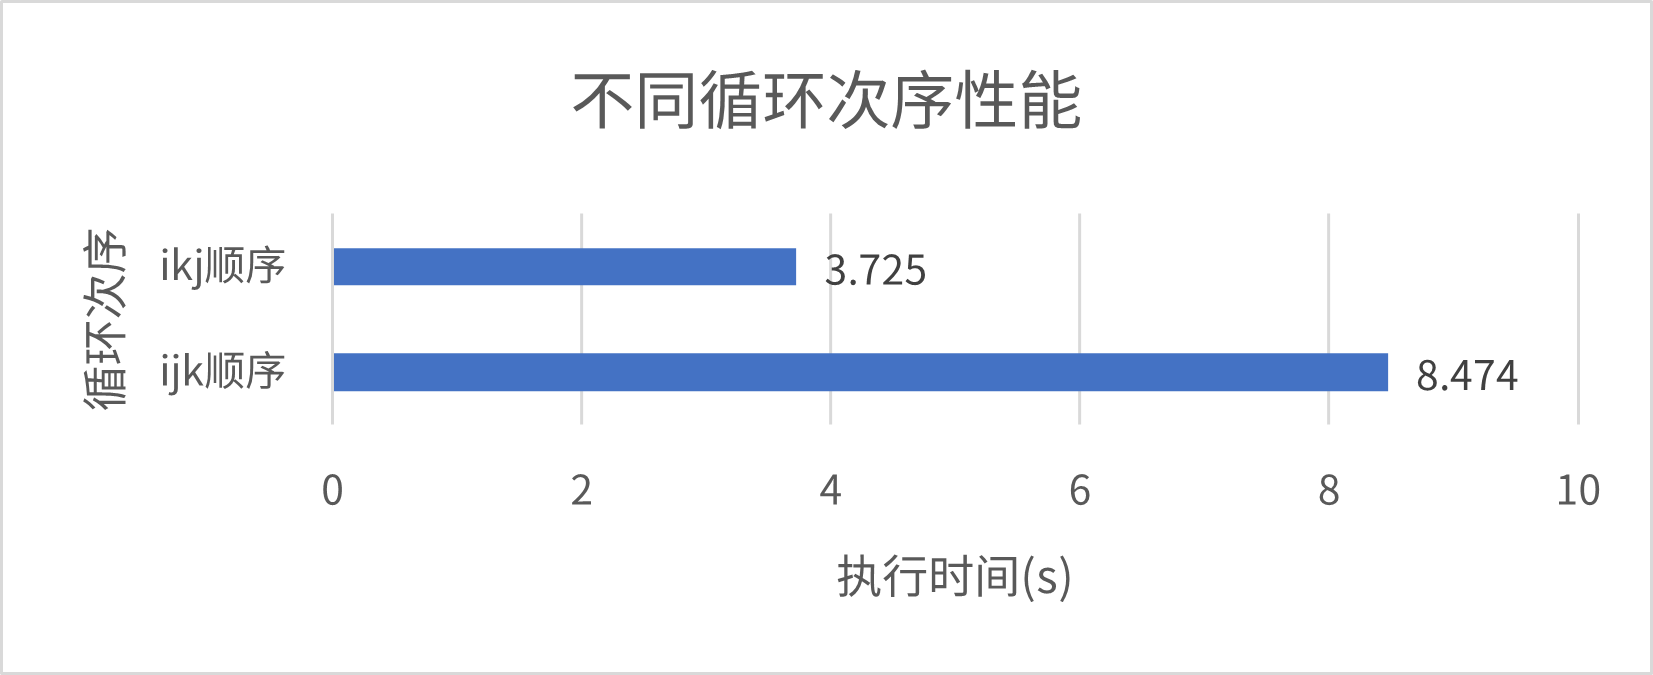
\includegraphics[width=0.9\textwidth]{cmp.png}
	\end{subfigure}
	\caption{结果}
	\label{fig:res}
\end{figure}

\subsection{分析}

矩阵在内存中常常以行优先的方式存储。因此,在\texttt{ijk}顺序中,对B的访问是按列的,会造成缓存不命中,性能降低。
而在\texttt{ikj}顺序中则调整成了按行访问,可以提高缓存命中率。
如图~\ref{fig:acc}。

\begin{figure}[htb]
	\centering
	\begin{subfigure}{0.4\textwidth}
		\centering
		\caption{\texttt{ijk}}
		\label{fig:ijkacc}
		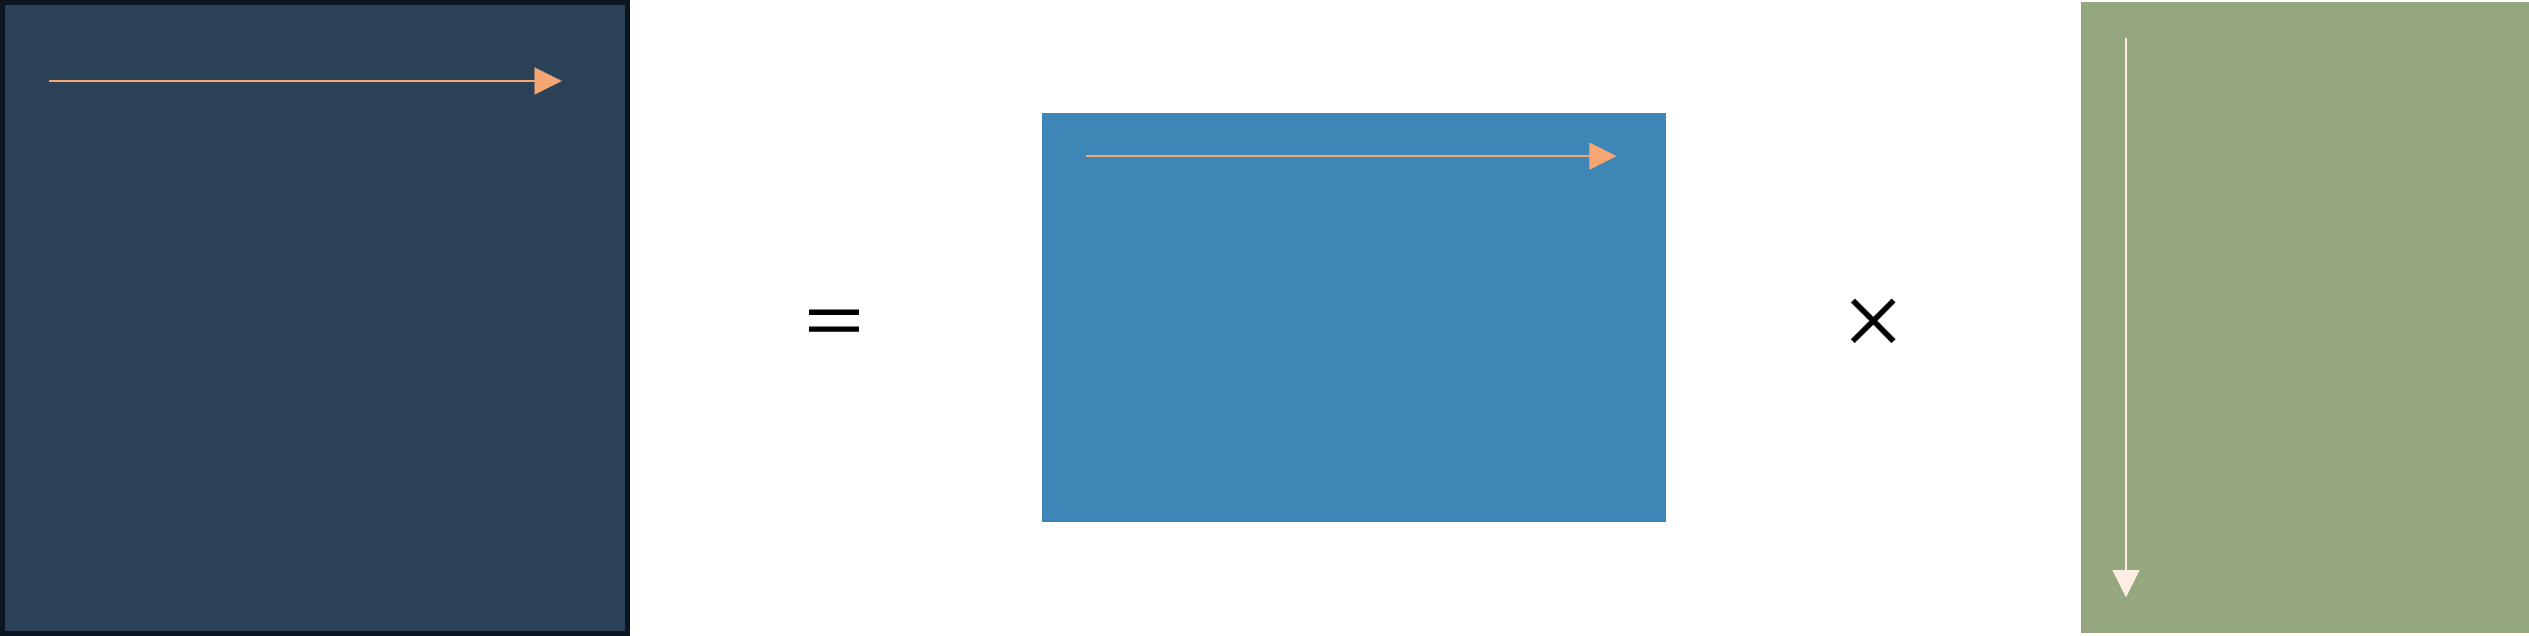
\includegraphics[width=0.9\textwidth]{acc.png}
	\end{subfigure}
	\begin{subfigure}{0.4\textwidth}
		\centering
		\caption{\texttt{ikj}}
		\label{fig:ikjacc}
		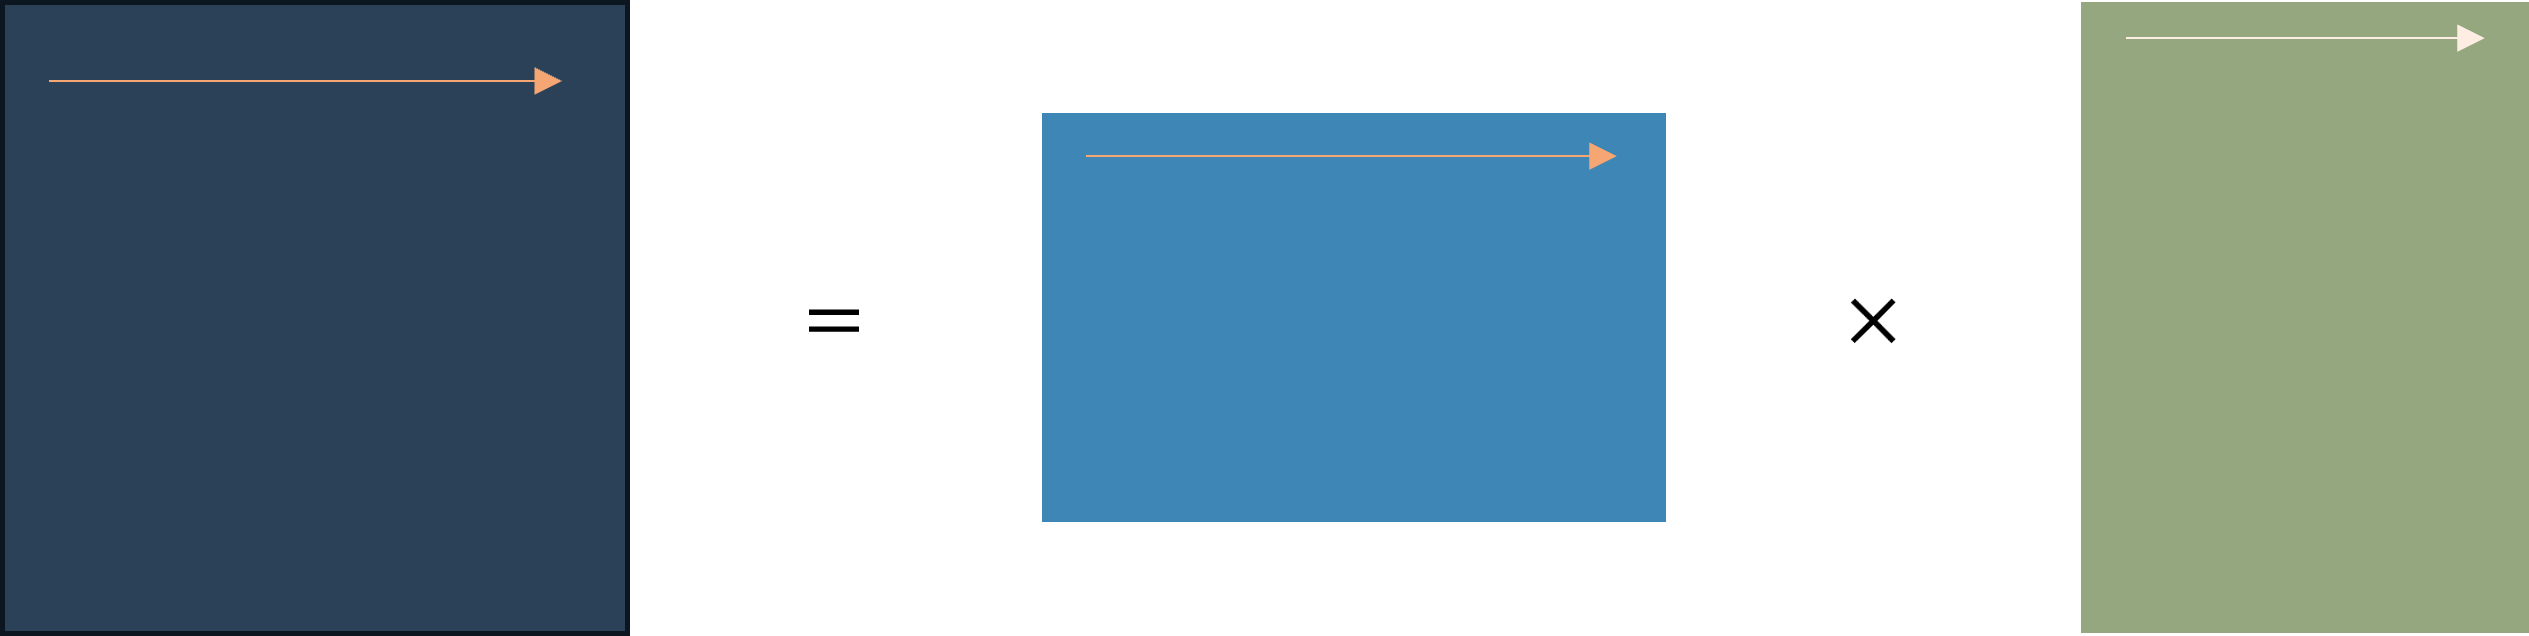
\includegraphics[width=0.9\textwidth]{acc2.png}
	\end{subfigure}
	\caption{访问方式}
	\label{fig:acc}
\end{figure}

然而,对C的访问虽然具有空间局部性,但缺乏时间局部性,因此如果缓存不够大或者相联程度比较低,这种方法可能不能提高性能。

\section{实验总结}

本次实验我探究了Cache的命中率与预取的关系,
然后通过调整循环次序探究了局部性对Cache命中率的影响,使得矩阵乘法得到了性能提升。
通过本次实验,加深了我对Cache的理解。

\end{spacing}

\end{document}